\part{Reactivity}


\chapter{Overview}


响应式系统(Reactivity System)和组件系统(Component System)是Vue 最显著的两个特性。

在Vue.js响应式系统中,模型层(model)只是普通 JavaScript 对象,修改它则更新视图(view),从而可以让状态管理变得非常简单且直观。


\section{Track Change}

把一个普通 Javascript 对象传给 Vue 实例的 data 选项,Vue 将遍历此对象所有的属性,并使用 Object.defineProperty 把这些属性全部转为 getter/setter。

Object.defineProperty 是仅 ES5 支持,且无法 shim 的特性,这也就是为什么 Vue 不支持 IE8 以及更低版本浏览器的原因。


用户看不到 getter/setter,但是在内部它们让 Vue 追踪依赖,在属性被访问和修改时通知变化。这里需要注意的问题是浏览器控制台在打印数据对象时 getter/setter 的格式化并不同,所以可能需要安装 vue-devtools 来获取更加友好的检查接口。

每个组件实例都有相应的 watcher 实例对象,它会在组件渲染的过程中把属性记录为依赖,之后当依赖项的 setter 被调用时,会通知 watcher 重新计算,从而致使它关联的组件得以更新。

\begin{figure}[htbp]
\centering
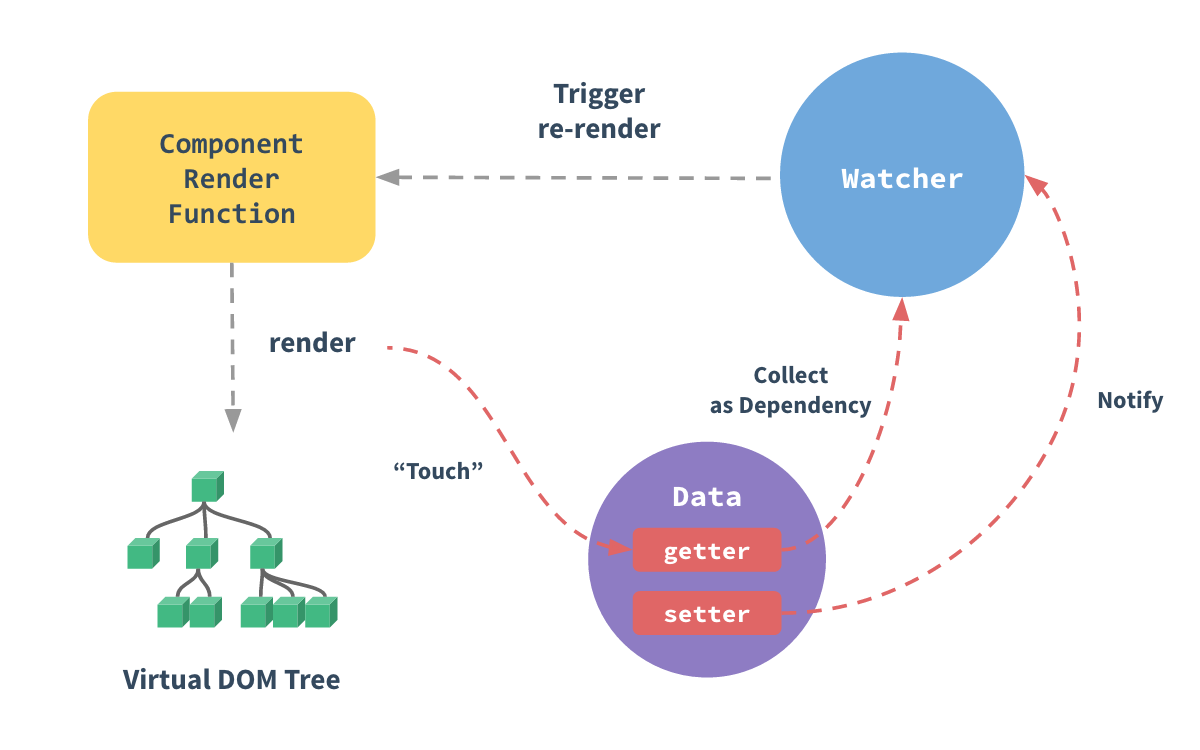
\includegraphics[scale=0.4]{data.png}
\caption{Vue响应式系统}
\end{figure}


\section{Detect Change}

受现代 Javascript 的限制(以及废弃 Object.observe),Vue 不能检测到对象属性的添加或删除。

由于 Vue 会在初始化实例时对属性执行 getter/setter 转化过程,所以属性必须在 data 对象上存在才能让 Vue 转换它,这样才能让它是响应式的。例如:



\begin{lstlisting}[language=JavaScript]
var vm = new Vue({
  data:{
  a:1
  }
})
// `vm.a` 是响应的
vm.b = 2
// `vm.b` 是非响应的
\end{lstlisting}

Vue 不允许在已经创建的实例上动态添加新的根级响应式属性(root-level reactive property),然而它可以使用 \texttt{Vue.set(object, key, value)} 方法将响应属性添加到嵌套的对象上:



\begin{lstlisting}[language=JavaScript]
Vue.set(vm.someObject, 'b', 2)
\end{lstlisting}

还可以使用 \texttt{vm.\$set}实例方法,这也是全局 Vue.set 方法的别名:



\begin{lstlisting}[language=JavaScript]
this.$set(this.someObject,'b',2)
\end{lstlisting}

有时需要向已有对象上添加一些属性,例如使用 Object.assign() 或 \_.extend() 方法来添加属性。但是,添加到对象上的新属性不会触发更新。在这种情况下可以创建一个新的对象,让它包含原对象的属性和新的属性:

\begin{lstlisting}[language=JavaScript]
// 代替 `Object.assign(this.someObject, { a: 1, b: 2 })`
this.someObject = Object.assign({}, this.someObject, { a: 1, b: 2 })
\end{lstlisting}


在列表渲染中也有一些数组相关的问题。




\begin{lstlisting}[language=JavaScript]

\end{lstlisting}



\begin{lstlisting}[language=JavaScript]

\end{lstlisting}






\begin{lstlisting}[language=JavaScript]

\end{lstlisting}



\begin{lstlisting}[language=JavaScript]

\end{lstlisting}






\begin{lstlisting}[language=JavaScript]

\end{lstlisting}



\begin{lstlisting}[language=JavaScript]

\end{lstlisting}


